\subsection{OB-17 (HWB)}
Princip útoků postranními kanály. Typy postranních kanálů, časový útok na porovnání polí, útok jednoduchou odběrovou analýzou (SPA) na šifru RSA.

\subsubsection*{Princip}
\begin{itemize}
	\item typy útoků:
	\begin{itemize}
		\item invazivní / semi-invazivní / neinvazivní (z hlediska fyzického průniku)
		\item pasivní / aktivní (jen odposlech, nebo i manipulace s rozhraním)
	\end{itemize}
	\item útoky postranními kanály jsou typicky pasivní a neinvazivní
	\item postranní kanál je výměna informace mezi kryptografickým modulem a jeho okolím, není to součást jeho normální funkce ale spíš vedlejší příznak způsobený slabinou fyzické či softwarové implementace
	\item postranním kanálem lze obejít matematické principy, na kterých je založena bezpečnost kryptografických operací
	\item často dovolí odhadovat klíč po částech
	
	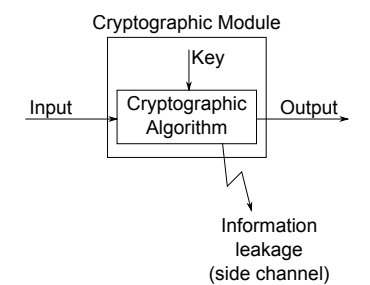
\includegraphics[width=0.5\textwidth]{img/OB-17_0.jpg}
\end{itemize}

\subsubsection*{Typy postraních kanálů}
\begin{itemize}
	\item časový postranní kanál --- doba vykonání operace závisí na tajemství, měřením času lze tajemství odhalit
	\item chybový postranní kanál --- chybový kód závisí na utajovaných datech
	\item odběrový postranní kanál (proudový / výkonový) ---  proudová spotřeba obvodu závisí na vnitřních datech v průběhu výpočtu šifry (simple/differential power analysis)
	\item elektromagnetický postranní kanál
	\item sociální kanál --- vyžaduje spolupráci uživatele
\end{itemize}

\subsubsection*{Časový útok na porovnání polí}
\begin{itemize}
	\item uvažujme 2 stejně velká pole, která chceme porovnat, dejme tomu zadané heslo vs správné heslo
	\item typicky porovnáváme po znacích/bytech, a když najdeme neshodu, končíme
	\item to je ale časový postranní kanál --- čím později porovnání skončí, tím více znaků od začátku je správně
	\item takto by správné heslo šlo hádat po znacích --- značně jednodušší než celé heslo naráz
	\item řešení: musí se vždy nějakým způsobem porovnat celé pole, tedy i když už víme že zadané heslo je špatné
\end{itemize}

\subsubsection*{Odběrový útok na RSA}
\begin{itemize}
	\item útok SPA --- Simple Power Analysis
	\item při dešifrování RSA dle vzorce $x = |c^d|_n$ se používá algoritmus Square and Multiply
	\item špatná implementace: square se provádí vždy (jednoduché, nízký odběr), a multiply se provádí jen  v případě, že aktuální bit je 1 (multiply je náročnější, vyšší odběr)
	\item v případě špatné implementace lze z odběru odhadnout, kdy se operace multiply prováděla a kdy ne, tedy sestavit bity tajné informace 
	
	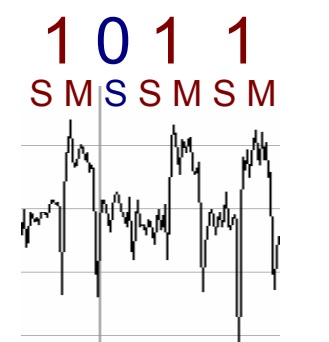
\includegraphics[width=0.5\textwidth]{img/OB-17_1.jpg}
	
	\item správná implementace: multiply se provede vždy, pokud ale výsledek není potřeba tak se zahodí
\end{itemize}

\subsubsection*{DPA}
\begin{itemize}
	\item Differential Power Analysis
	\item mnoho průběhů, provádí se analýza signálu ve stejných okamžicích napříč všemi průběhy
	\item dále se předgenerují všechny možné hodnoty klíče, na základě toho také hypotetické spotřeby průběhů
	\item z hypotetických průběhů se najde ten, co nejvíce odpovídá reálným průběhům --- klíč odhalen
\end{itemize}